% --------------------------------------------------------------------------------

\begin{exercise}

Zeigen Sie, dass

\begin{align*}
  F = \frac{1}{\sigma_n}\frac{x}{|x|^n}
\end{align*}

eine Fundamentallösung des Differentialoperators $L(u) = \Div(u)$ auf $\R^n$ ist, wobei $\sigma_n$ die Oberfläche der Einheitskugel im $\R^n$ ist.
Achtung:
Obwohl $F$ eigentlich eine vektorwertige Distribution in $L_{\mathrm{loc}}^1(\R^n)^n$ ist, wird das nicht gebraucht um die Behauptung

\begin{align*}
  \abraces{\Div F, \varphi} = \varphi(0)
\end{align*}

zu zeigen, da $\Div F = \frac{1}{\sigma_n}\sum_{i} \partial_i \pbraces{\frac{x_i}{|x|^n}} \in \mathcal{D}^{\prime}(\R)$ ist.
\end{exercise}

% --------------------------------------------------------------------------------

\begin{solution}

\phantom{}

\begin{figure}[h!]
  \centering
  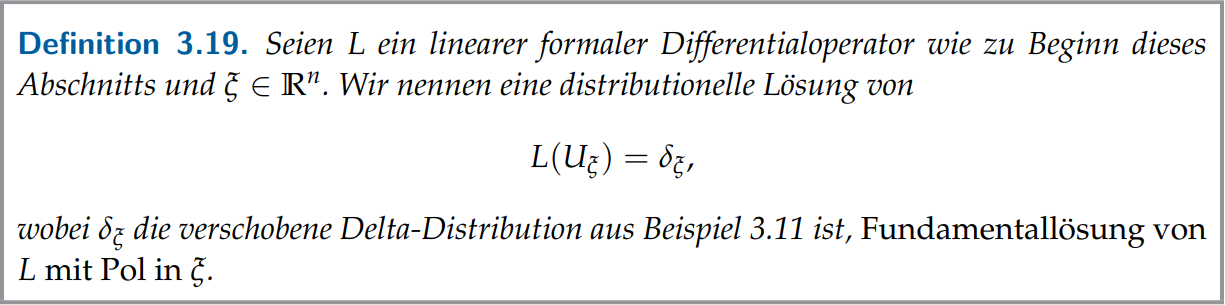
\includegraphics
  [width = 0.75 \textwidth]
  {Definition 3-19.png}
\end{figure}

Sei $\phi \in \mathcal{D}(\R^n)$.
Wir wollen im Folgenden partiell integrieren.

\includegraphicsboxed
{Analogon der partiellen Integration.png}

Die Partielle Integration basiert auf dem Integral-Satz von Gauß.
Um diesen anzuwenden, brauchen wir eine offene und beschränkte Menge.
Das garantieren wir formal, indem wir $\Omega \supseteq \supp(\phi)$ als offene und beschränkte Menge mit $C^1$-Rand wählen und durch $\Omega_\epsilon := \Omega \setminus \overline{B_\epsilon(0)}$ für $\epsilon > 0$ die Singularität $0$ rausschneiden.
Wir integrieren somit nur auf $\Omega$ bzw. $\Omega_\epsilon$.
(Außerhalb des Trägers, verschwindet alles).

\begin{align*}
  \implies
  \abraces{L F, \phi}
  & =
  \abraces{\Div F, \phi}
  =
  \abraces
  {
    \frac{1}{\sigma_n}
    \sum_{i = 1}^n
    \partial_i
    \pbraces
    {
      \frac{x_i}{|x|^n}
    },
    \phi
  }
  =
  \frac{1}{\sigma_n}
  \sum_{i=1}^n
  \abraces
  {
    \partial_i
    \pbraces
    {
      \frac{x_i}{|x|^n}
    },
    \phi
  }
  =
  -\frac{1}{\sigma_n}
  \sum_{  1}^n
  \abraces
  {
    \frac{x_i}{|x|^n},
    \partial_i \phi
  } \\
  & =
  -\frac{1}{\sigma_n}
  \abraces
  {
    \sum_{i=1}^n
    \frac{x_i}{|x|^n},
    \partial_i \phi
  }
  =
  -\frac{1}{\sigma_n}
  \Int[\Omega]
  {
    \sum_{i = 1}^n
    \frac{x_i}{|x|^n}
    \partial_i \phi
  }{x}
  =
  -\frac{1}{\sigma_n}
  \Int
  [\Omega]
  {
    \frac{x}{|x|^n}
    \cdot
    \nabla \phi(x)
  }{x} \\
  & =
  \lim_{\epsilon \to 0^+}
  -\frac{1}{\sigma_n}
  \Int
  [\Omega_\epsilon]
  {
    \frac{x}{|x|^n}
    \cdot
    \nabla \phi(x)
  }{x}
  \stackrel{\text{PI}}{=}
  \lim_{\epsilon \to 0^+}
  \frac{1}{\sigma_n}
  \pbraces
  {
    \Int
    [\Omega_\epsilon]
    {
      \Div
      \pbraces
      {
        \frac{x}{|x|^n}
      }
      \phi(x)
    }{x}
    -
    \Int
    [\partial \Omega_\epsilon]
    {
      \frac{x}{|x|^n}
      \phi(x)
      \cdot
      \nu
    }{s}
  } \\
  & =
  \lim_{\epsilon \to 0^+}
  \frac{1}{\sigma_n}
  \Bigg (
    \Int
    [\Omega_\epsilon]
    {
      \Div
      \pbraces
      {
        \frac{x}{|x|^n}
      }
      \phi(x)
    }{x}
    -
    \underbrace
    {
      \Int
      [\partial \Omega]
      {
        \frac{x}{|x|^n}
        \phi(x)
        \cdot
        \nu
      }{s}
    }_0
    -
    \Int
    [\partial B_\epsilon(0)]
    {
      \frac{x}{|x|^n}
      \phi(x)
      \cdot
      \nu
    }{s}
  \Bigg )
\end{align*}

Wir kümmern uns nun um die übrigen Integrale separat.
Das Erste fällt weg, weil

\begin{align*}
  \mathrm{div}\left(\frac{x}{|x|^n}\right)
  =\frac{1}{\sigma_n}\sum_{i=1}^n\partial_i\left(\frac{x_i}{|x|^n}\right)
  &= \frac{1}{\sigma_n}\sum_{i=1}^n\frac{\left(\sum_{i=1}^nx_i^2\right)^{n/2} - x_i2x_i\frac{n}{2}\left(\sum_{i=1}^nx_i^2\right)^{n/2 - 1}}{\left(\sum_{i=1}^nx_i^2\right)^n} \\
  &= \frac{1}{\sigma_n}\sum_{i=1}^n\frac{1 - \frac{nx_i^2}{\sum_{i=1}^nx_i^2}}{\left(\sum_{i=1}^nx_i^2\right)^{n/2}} \\
  &= \frac{1}{\sigma_n}\frac{n - n\frac{\sum_{i=1}^nx_i^2}{\sum_{i=1}^nx_i^2}}{\left(\sum_{i=1}^nx_i^2\right)^{n/2}} = 0.
\end{align*}

Das Zweite wird zu genau dem Rest, den wir brauchen.
Dazu bemerken wir, dass das Normalvektorfeld auf $\partial B_\epsilon(0)$ wie folgt aussieht.

\begin{align*}
  |x| = \epsilon,
  \quad
  \nu(x)
  =
  -\frac{x}{|x|}
\end{align*}

Mit dem Mittelwertsatz der Integralrechnung berechnen wir den Rest.

\begin{multline*}
  -\Int
  [\partial B_\epsilon(0)]
  {
    \frac{x}{|x|^n}
    \phi(x)
    \cdot
    \nu
  }{s}
  =
  \Int
  [\partial B_\epsilon(0)]
  {
    \frac{x \cdot x}{|x|^{n+1}}
    \phi(x)
  }{s}
  =
  \Int
  [\partial B_\epsilon(0)]
  {
    \frac{|x|^2}{|x|^{n+1}}
    \phi(x)
  }{s}
  =
  \Int
  [\partial B_{\epsilon}(0)]
  {
    \frac{\epsilon^2}{\epsilon^{n+1}}
    \phi(x)
  }{s} \\
  \stackrel{\text{MWS}}{=}
  \epsilon^{1-n}
  \phi(x_\epsilon)
  \meas \partial B_{\epsilon}(0)
  =
  \epsilon^{1-n}
  \epsilon^{n-1}
  \sigma_n
  \phi(x_\epsilon)
  =
  \sigma_n
  \phi(x_{\epsilon})
\end{multline*}

Formal gilt noch zu zeigen, dass $F_i = \frac{x_i}{|x|^n}$ eine $L^1_{\mathrm{loc}}$-Funktion ist, dazu betrachten wir
das Integral über den Radialanteil in sphärischen Koordinaten. Dort betrachten wir eine Kugel die unser Kompaktum umfasst. Dann gilt
für $g(x) = |x|^{1-n}$, da $r = |x|$

\begin{align*}
  \int_0^r z^{1-n}z^{n-1} dz = r
  <
  \infty
\end{align*}

Damit ist nach folgender Rechnung auch $\sum_{i=1}^n |F_i|$, und somit auch $F_i$ eine $L^1_{\mathrm{loc}}$-Funktion.

\begin{align*}
  \Int[K]
  {
    \sum_{i=1}^n\frac{|x_i|}{|x|^n}
  }{x}
  \stackrel{CS}{\leq}
  \Int[K]
  {
   n \frac{|x|}{|x|^n}
  }{x}
  =
  n\Int[K]
  {
    |x|^{1-n}
  }{x}
  <
  \infty
\end{align*}

\end{solution}

% --------------------------------------------------------------------------------
